\documentclass{standalone}
\usepackage{tikz}
\begin{document}

    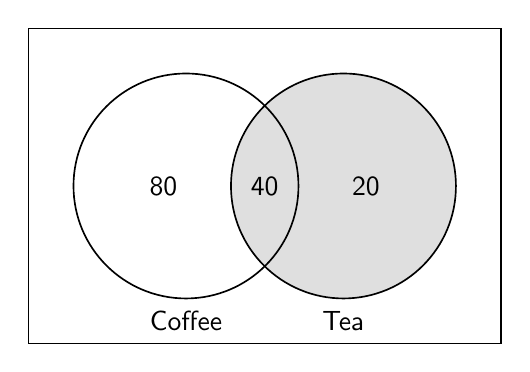
\begin{tikzpicture}[scale=2/7,font=\sffamily]
        \draw[semithick] (0,0) rectangle (21,14);

        % Sets: Path is fill, draw is bddry
        \path[fill=white] (7,7) circle (5);
        \path[fill=gray!25] (14,7) circle (5);
        \draw[semithick] (7,7) circle (5);
        \draw[semithick] (14,7) circle (5);

        % Set names
        \node at (7,1) {Coffee};
        \node at (14,1) {Tea};

        % Numbers in each region
        \node at (6,7) {80};  % Only in X
        \node at (10.5,7) {40};    % Intersection
        \node at (15,7) {20};   % Only in Y
    \end{tikzpicture}

\end{document}